\section{Background}

\begin{figure}[t!]
    \centering
    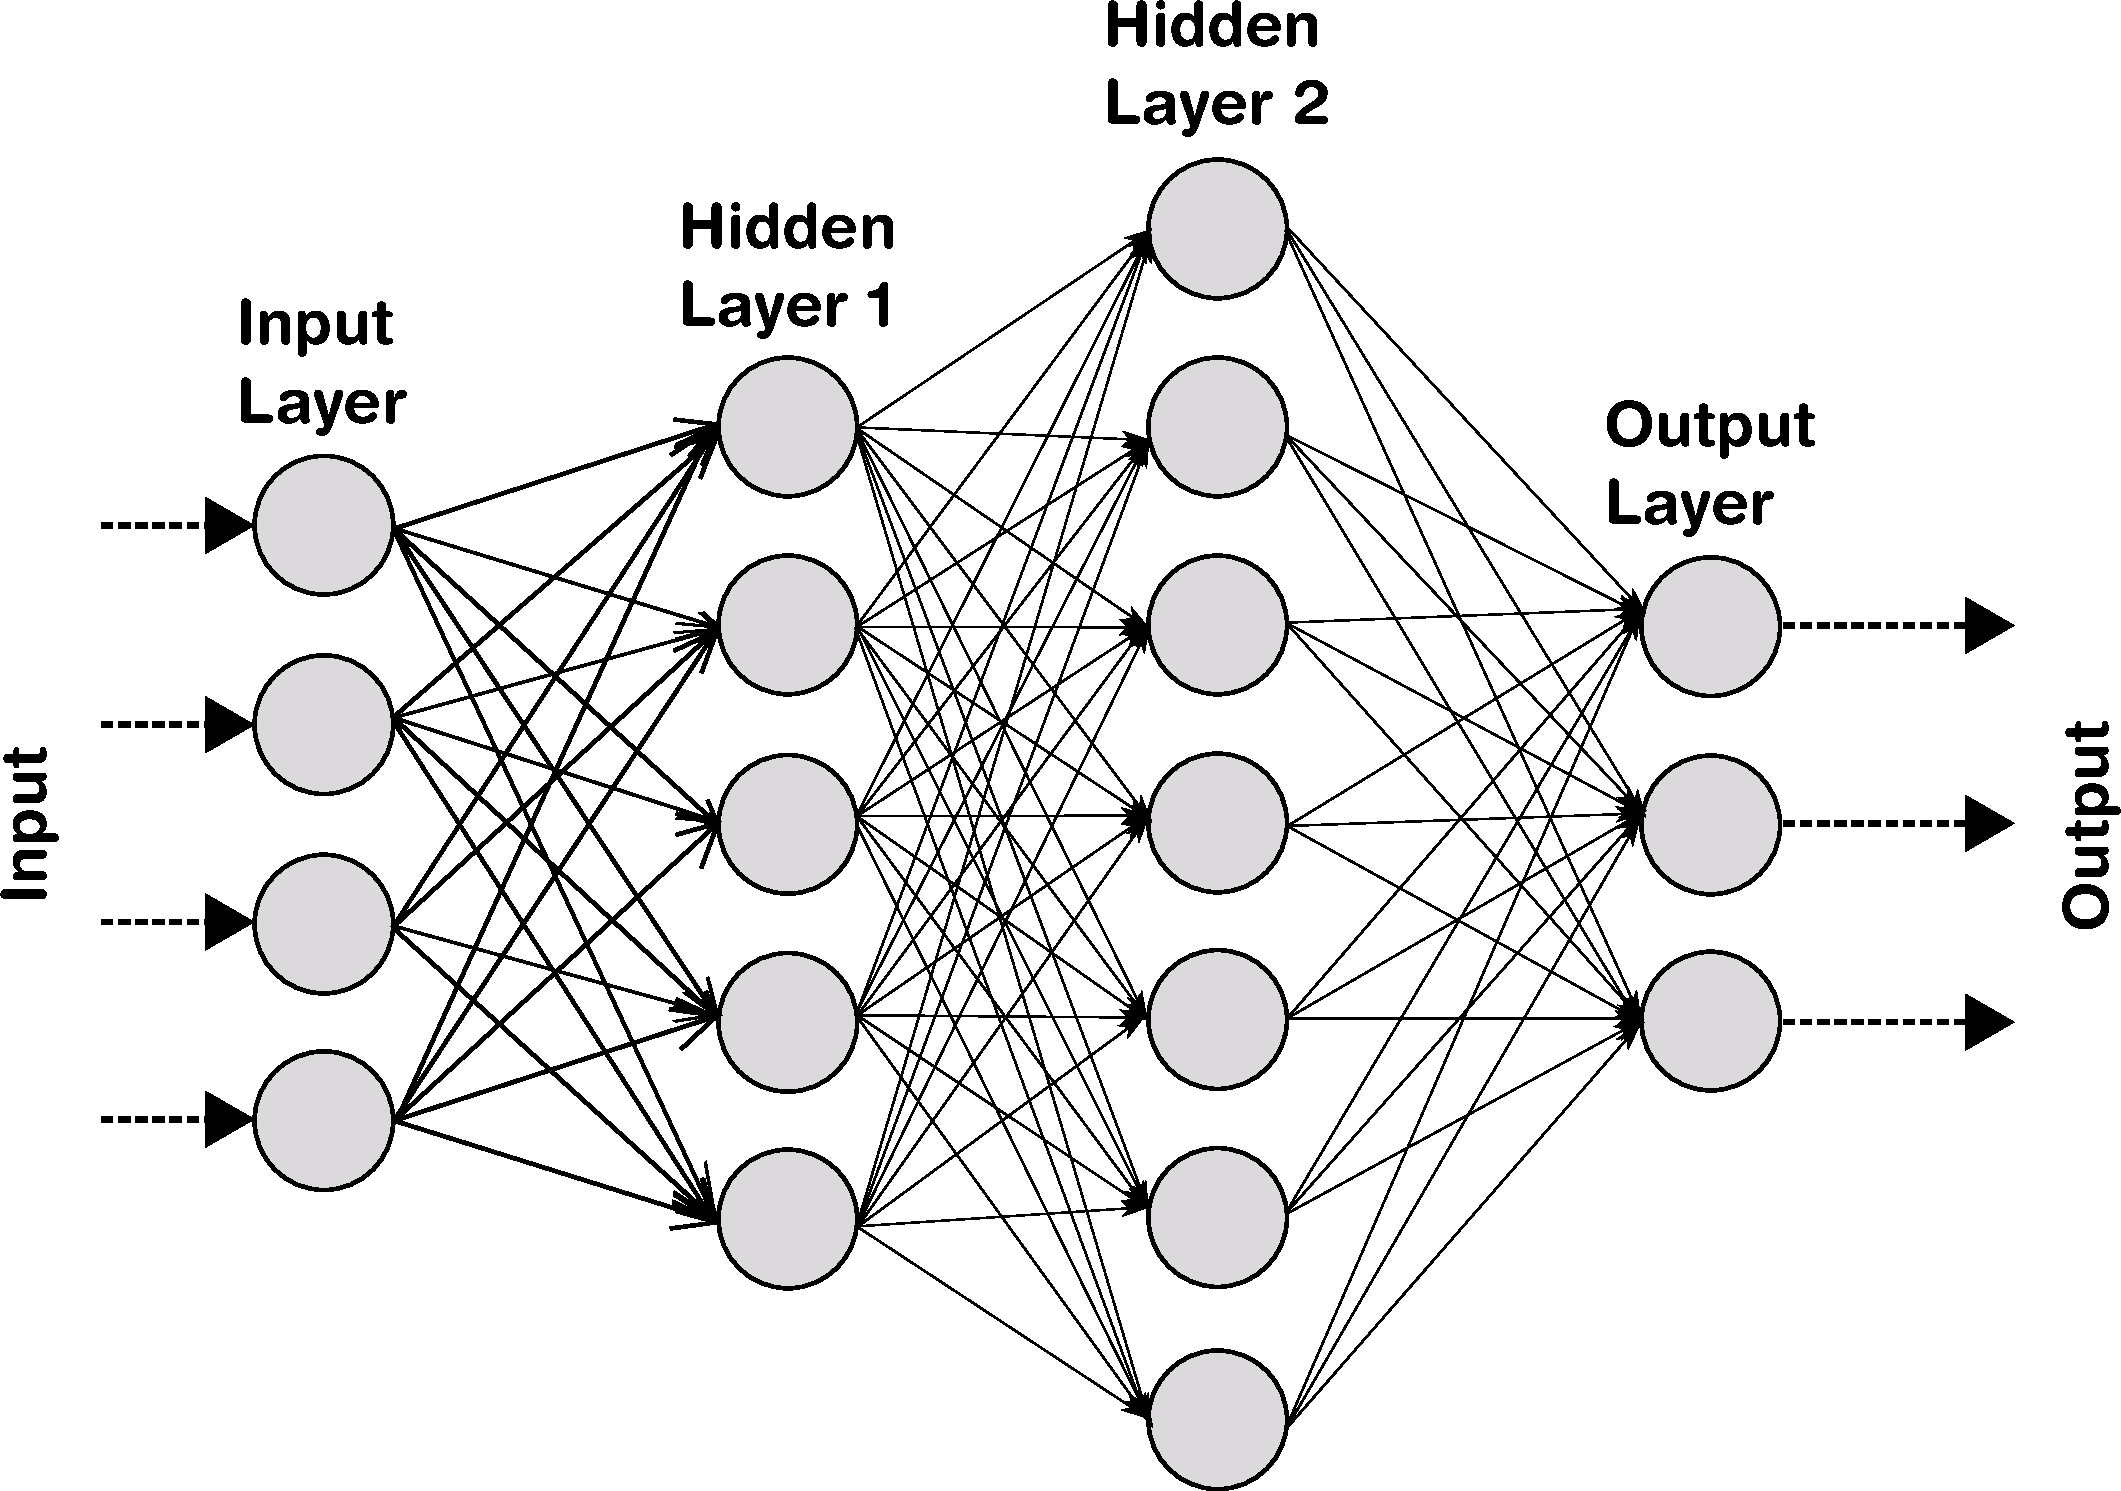
\includegraphics[width = 0.8\columnwidth]{Figures/NeuralNetwork.pdf}
    \caption{Caption}
    \label{fig:my_label}
\end{figure}


~\cite{Furber2013}
ANN is an inspired and adapted model of biological brain. Network consists of many layers, where each layer is constructed form several neurons. The signal transition takes place between neurons through synapse. Each synapse has its own weight, which affects the signal passing though it: the signal is multiplied by the weight of the corresponding synapse. The inputs to the neuron from the synapses are summed up in the neuron and passed further to the activation function. Activation function transforms the input signals to output signals, and its main function is to make decision regarding how the output should behave to certain inputs. Fig. depicts the neuron with the basic operations it performs. 


\begin{figure}[t!]
    \centering
    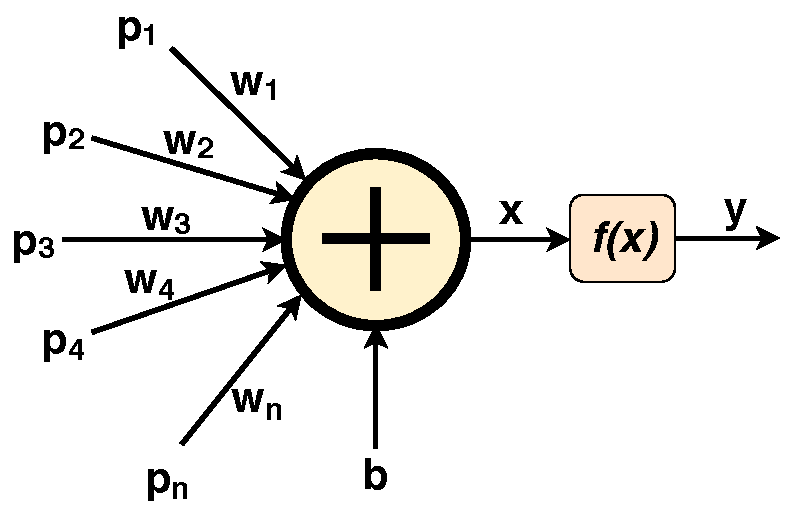
\includegraphics[width = 0.3\textwidth]{Figures/ANN.pdf}
    \caption{Caption}
    \label{fig:my_label}
\end{figure}

ANN can consist of many layers, which are classified into three groups: input layer, hidden layer and output layer. One layer can be fully or partially connected to the next layer. Hidden layer can be built from many intermediate layers between input an output. 

\subsection*{Number Representation}

One critical factor in hardware implementation of ANN is the number representation of different data - synapse weights, biases and inputs/outputs of the neurons. Despite its widely usage in software ANNs, floating point arithmetic due to its prohibitively expensive cost is not well suited for hardware ANNs. As a result, the two's complement fixed binary point representation was chosen for data representation as it brings considerable optimization in terms of area usage and speed performance. However, this implies limited precision which is enough for many applications. Nevertheless, with this scheme learning process is accomplished off-chip in software using floating point representation. The conversions from decimal fractions to fixed point binary is done through equation~\ref{equation:dtob}.

\begin{equation}
b_{x}(d_{x})= \lfloor{d_{x}\cdot \frac{2^{n_{x}-1}-1}{2^{i_{x}-1}-2^{-f_{x}}}}\rceil
\label{equation:dtob}
\end{equation}
\begin{equation}
d_{x}(b_{x})= {b_{x}\cdot \frac{2^{i_{x}-1}-2^{-f_{x}}}{2^{n_{x}-1}-1}}
\label{equation:btod}
\end{equation}
Here, $n_{x}$, ${x}$, $f_{x}$ amount to total number of bits, integer bits and fractional bits of the given variable.
